\chapter{局域量子場與一維狄拉克方程}

我們已透過量子場的量子、產生與湮滅算符，以及非相對論粒子的最簡哈密頓量，認識了量子場。現在要讓這套架構發揮作用。首先，我們要實際看見空間局域的哈密頓量如何守恆動量，而不只是提出這項主張。接著，我們會讓場的乘積描述散射與衰變，並觀察哈密頓量反覆作用如何展現圖形化微擾理論的雛形。之後才會轉向先前預告的費米子問題。最直接的切入點還不是費米子場，而是一維狄拉克方程。

\section{再談場的哈密頓量}

把一種非相對論粒子的哈密頓量寫成
\begin{equation}
H_0=\int dx\,
\psi^\dagger(x)
\left[-\frac{\partial_x^2}{2m}+V(x)\right]
\psi(x).
\label{eq:l9-nonrel-hamiltonian}
\end{equation}
這些記號看起來是一維的，但接下來的初步論證並不依賴這項限制：在三維中，\(x\)可以代表向量\(\mathbf{x}\)，\(dx\)代表\(d^3x\)，而\(-\partial_x^2\)代表\(-\nabla^2\)。

算符\(\psi^\dagger(x)\)在\(x\)處產生一個粒子，而\(\psi(x)\)則在該處湮滅一個粒子。它們的正規序乘積
\begin{equation}
n(x)=\psi^\dagger(x)\psi(x)
\end{equation}
就是局域數密度。因此，勢能項為
\begin{equation}
H_V=\int dx\,V(x)n(x).
\end{equation}
這正是描述經典氣體時會寫下的形式：數出\(x\)附近的粒子，為每個粒子指定勢能\(V(x)\)，再對整個空間加總。在這個階段，粒子彼此並不相互作用。它們可以受到外加勢的影響，但除此之外，哈密頓量就是各個獨立單粒子能量的總和。

我們不妨先簡化問題，再回到原來的情況。令勢能為常數\(V(x)=V_0\)。常數勢不會施力，但它的算符意義十分明確：
\begin{equation}
\begin{aligned}
H_V&=V_0\int dx\,\psi^\dagger(x)\psi(x)=V_0N,\\
N&=\int dx\,n(x).
\end{aligned}
\end{equation}
它為每個粒子加上相同的能量。若要在非相對論描述中保留靜止能量，就取\(V_0=mc^2\)。如此一來，這一項便為每個粒子計入一份靜止能量。我們保留這個原本乏味的常數，因為它維持平移不變性，也讓粒子數的計算清楚可見。

\section{哈密頓量作為更新規則}

動量守恆究竟是什麼意思？我們應從哈密頓量如何作用來說明。為了避免同時用\(\psi\)表示場算符、單粒子波函數與多體態，以下把多體態記為\(\lvert\Phi(t)\rangle\)。在一段短時間\(\epsilon\)內，
\begin{equation}
\lvert\Phi(t+\epsilon)\rangle
=\left(1-i\epsilon H+O(\epsilon^2)\right)
\lvert\Phi(t)\rangle,
\label{eq:l9-short-update}
\end{equation}
其中\(\hbar=1\)。第一項是未改變的狀態；第一個修正項由\(H\)產生。反覆施行這項更新，就得到Schr\"odinger方程。

現在，動量守恆有了具體意義。如果初始態具有確定的總動量\(P\)，那麼\(H\lvert\Phi\rangle\)也必須具有相同的總動量。其他性質可能改變，個別粒子也可能彼此交換動量，但哈密頓量不能讓狀態進入總\(P\)不同的子空間。我們可以直接在動量基底中改寫哈密頓量，檢驗這一點。

\section{空間積分如何產生動量狄拉克{\proseunicodefont δ}函數}

採用以下傅立葉轉換約定
\begin{align}
\psi(x)&=\int\frac{dp}{\sqrt{2\pi}}\,a(p)e^{ipx},\\
\psi^\dagger(x)&=\int\frac{dq}{\sqrt{2\pi}}\,a^\dagger(q)e^{-iqx}.
\label{eq:l9-field-fourier}
\end{align}
算符\(a(p)\)湮滅一個動量為\(p\)的粒子；算符\(a^\dagger(q)\)則產生一個動量為\(q\)的粒子。兩者必須使用不同的字母：在空間積分將兩個動量聯繫起來之前，它們是彼此獨立的積分變數。

先看粒子數項：
\begin{align}
N
&=\int dx\,\psi^\dagger(x)\psi(x)\\
&=\int\frac{dp\,dq}{2\pi}\,
a^\dagger(q)a(p)
\int dx\,e^{i(p-q)x}.
\end{align}
剩下的積分是
\begin{equation}
\int dx\,e^{i(p-q)x}=2\pi\delta(p-q).
\end{equation}
當\(p\ne q\)時，相位會振盪，正負貢獻彼此抵消；當\(p=q\)時，相位則完全不振盪。狄拉克{\proseunicodefont δ}分布正是精確表達這兩項事實的數學對象。因此，
\begin{align}
N
&=\int dp\,dq\,a^\dagger(q)a(p)\delta(p-q)\\
&=\int dp\,a^\dagger(p)a(p).
\label{eq:l9-number-momentum}
\end{align}
這個算符湮滅一個動量為\(p\)的粒子，再產生一個動量完全相同的粒子。關鍵在於對\(x\)積分：它產生的{\proseunicodefont δ}函數會強制入射與出射動量相等。

\begin{classroomqa}
\lecturetimestamp{00:17:02}
\audiencequestion{當\(p=q\)時出現的無窮大去哪裡了？}
\lecturerresponse{{\proseunicodefont δ}函數不是藉由取其高度來使用的；它是由積分定義的分布：\(\int dk\,\delta(k)f(k)=f(0)\)。``無限高且無限窄''這種說法只是提醒我們，它的積分權重為一。在這裡，{\proseunicodefont δ}函數告訴我們令\(p-q=0\)，因此不會留下任何無窮大的結果。}
\end{classroomqa}

相同的機制也適用於更一般的局域單項式。假設某一項含有數個湮滅場與數個產生場；它們可能屬於不同種類，但都在同一點取值，並對該點積分：
\begin{equation}
\int dx\,
\prod_{r=1}^{n} \psi_{i_r}^\dagger(x)
\prod_{s=1}^{m} \psi_{j_s}(x).
\end{equation}
令被湮滅粒子的動量為\(p_s\)，被產生粒子的動量為\(q_r\)。經過傅立葉展開後，得到
\begin{equation}
\int dx\,
e^{i(\sum_s p_s-\sum_r q_r)x}
=2\pi\,
\delta\!\left(\sum_s p_s-\sum_r q_r\right).
\label{eq:l9-total-momentum-delta}
\end{equation}
結果不會將\(p_1\)與\(q_1\)配成一對、將\(p_2\)與\(q_2\)配成一對，依此類推；它只要求
\begin{equation}
\sum_{\mathrm{annihilated}}p
=
\sum_{\mathrm{created}}q.
\end{equation}
這正是相互作用所需的規則：個別動量可以改變，但總動量不變。更深一層的說法是平移不變性。局域密度在每一點都以相同權重積分，因此沒有偏好的原點；其傅立葉變換便帶有相應的動量守恆{\proseunicodefont δ}函數。

\begin{classroomqa}
\lecturetimestamp{00:23:04}
\audiencequestion{所提出的哈密頓量項真的由所有那些場算符相乘而成嗎？我們為什麼要寫下這種乘積？}
\lecturerresponse{是的。這個乘積指定哪些粒子在同一點被湮滅、哪些粒子在該處產生。它的物理動機將來自觀測到的散射或衰變過程；我們先建立動量守恆的論證，之後就能直接看出這些相互作用的意義。}
\end{classroomqa}

\section{動量空間與位置空間中的動能}

現在用同一套方法處理導數項。導數作用在平面波上：
\begin{equation}
-\partial_x^2 e^{ipx}=p^2e^{ipx}.
\end{equation}
因此
\begin{align}
H_{\mathrm{kin}}
&=\int dx\,\psi^\dagger(x)
\left(-\frac{\partial_x^2}{2m}\right)\psi(x)\\
&=\int dp\,\frac{p^2}{2m}\,a^\dagger(p)a(p).
\label{eq:l9-kinetic-momentum}
\end{align}
空間積分再次強制入射與出射動量相等。新的因子\(p^2/2m\)只是在每個動量模式的粒子數前乘上該模式的動能，作為權重。

\begin{classroomqa}
\lecturetimestamp{00:24:46}
\audiencequestion{對平面波微分兩次，結果不應該帶負號嗎？}
\lecturerresponse{是的，\(\partial_x^2e^{ipx}=-p^2e^{ipx}\)。哈密頓量本身已含有抵消該負號的負號，所以\(-\partial_x^2\)的本徵值為正，等於\(p^2\)。}
\end{classroomqa}

\begin{classroomqa}
\lecturetimestamp{00:27:20}
\audiencequestion{只有勢能為常數時，動能才守恆嗎？}
\lecturerresponse{是的。若沒有隨位置改變的勢能，就沒有作用力，動能本身會守恆。在非定值的外加勢中，動能與勢能可以彼此轉換；只要總哈密頓量沒有明確的時間依賴，總能量仍然守恆。}
\end{classroomqa}

\begin{classroomqa}
\lecturetimestamp{00:27:42}
\audiencequestion{在動量空間的動能哈密頓量中，\(\psi^\dagger\psi\)扮演什麼角色？}
\lecturerresponse{它是計數算符。模式乘積\(a^\dagger(p)a(p)\)計算動量為\(p\)的粒子數，而因子\(p^2/2m\)則為每個粒子指定相應的動能。}
\end{classroomqa}

還有另一種看出動能為非負的方法。分部積分一次並略去邊界項，可得
\begin{align}
\int dx\,\psi^\dagger(-\partial_x^2)\psi
&=\int dx\,(\partial_x\psi^\dagger)(\partial_x\psi).
\label{eq:l9-positive-kinetic}
\end{align}
對於在無窮遠處適當趨近於零的場，或採用週期邊界條件時，邊界項為零。所得形式是絕對值的平方，因此非負。這也呈現場論中常見的形式：能量包含場的空間導數平方。

\section{局域接觸相互作用}

現在讓場的乘積派上用場。考慮兩種粒子，為了讓例子容易理解，我們姑且稱它們為電子與質子。目前這只是刻意簡化的模型：兩者都以玻色子算符描述，並且暫不納入真實存在的庫侖相互作用。它們的自由哈密頓量是
\begin{equation}
H_0=\int dx\left[
\psi_e^\dagger\left(-\frac{\partial_x^2}{2m_e}\right)\psi_e
+
\psi_p^\dagger\left(-\frac{\partial_x^2}{2m_p}\right)\psi_p
\right].
\end{equation}
再加入模型中的相互作用項
\begin{equation}
H_{\mathrm{contact}}
=g\int dx\,
\psi_e^\dagger(x)\psi_p^\dagger(x)
\psi_e(x)\psi_p(x).
\label{eq:l9-contact}
\end{equation}
由右向左讀這個算符：它在同一位置\(x\)找出一個電子和一個質子，將兩者湮滅，再在該處重新產生。如果兩個粒子不在一起，這個局域項的作用為零。如果它們的世界線相交，這一項就可能改變個別粒子的動量，同時保留總動量。因此，它描述的是理想化的零程散射勢。

\begin{figure}[htbp]
\centering
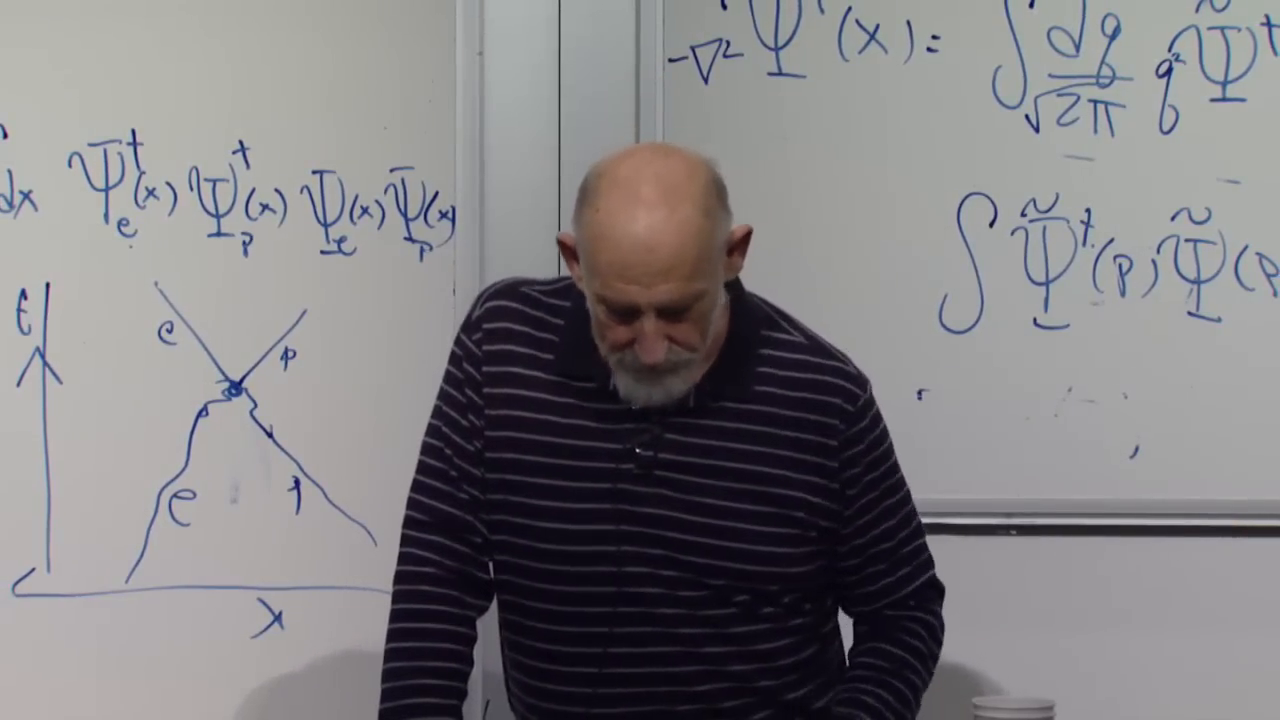
\includegraphics[width=0.94\linewidth]{lecture_09_frame_02.png}
\caption{黑板上的接觸相互作用。時空示意圖上方列出四個局域場算符；這個理想化相互作用只在粒子相遇處作用。}
\lectureframe{00:35:36}
\end{figure}

\begin{figure}[htbp]
\centering
\begin{tikzpicture}[x=1.2cm,y=1.0cm,>=Latex]
\draw[->] (-3.0,0) -- (3.0,0) node[right] {$x$};
\draw[->] (0,-0.2) -- (0,4.2) node[above] {$t$};
\coordinate (v) at (0,2.0);
\fill (v) circle (1.8pt);
\draw[thick,->] (-2.2,0.4) -- (v);
\draw[thick,->] (2.0,0.4) -- (v);
\draw[thick,->] (v) -- (-1.6,3.7);
\draw[thick,->] (v) -- (2.2,3.7);
\node[left] at (-1.65,0.7) {$e$};
\node[right] at (1.55,0.7) {$p$};
\node[left] at (-1.15,3.3) {$e$};
\node[right] at (1.65,3.3) {$p$};
\node[right] at (0.12,2.05) {$g$};
\end{tikzpicture}
\caption{局域散射圖像的清楚重繪。這個頂點是式~\eqref{eq:l9-contact}所示算符的簡寫，不是經典碰撞定律。}
\end{figure}

真實的電子與質子會透過庫侖勢在彼此尚有距離時相互作用。接觸模型只是初步的簡化：如果實驗顯示兩種粒子只有在空間重疊時才會散射，我們就會把類似式~\eqref{eq:l9-contact}的項放進哈密頓量。

\begin{classroomqa}
\lecturetimestamp{00:35:40}
\audiencequestion{如果能量沒有改變，為什麼散射算符會是哈密頓量的一部分？}
\lecturerresponse{哈密頓量既是能量算符，也是產生狀態變化的生成元。兩個粒子之間的勢能會在時間演化中造成散射。總能量守恆，並不表示狀態或個別粒子的動量保持不變。}
\end{classroomqa}

這帶出一條實用原則：先從實驗了解粒子可能經歷哪些局域過程，再用更新狀態的算符將這些過程寫進理論。場的乘積不是純粹裝飾性的代數；其中帶有伴隨符號與不帶伴隨符號的因子，指定了哪些種類的粒子出現或消失。

\section{衰變、逆過程與厄米性}

假設氣泡室中有一條粒子種類\(A\)的徑跡在某點終止，並從該點出現粒子\(B\)與\(C\)的徑跡。這個局域過程是
\begin{equation}
A\longrightarrow B+C.
\end{equation}
實現這個過程的算符是
\begin{equation}
V=g\int dx\,
\psi_B^\dagger(x)\psi_C^\dagger(x)\psi_A(x).
\label{eq:l9-decay-half}
\end{equation}
湮滅場移除\(A\)；兩個產生場則在同一位置產生\(B\)與\(C\)。以相同權重對每個\(x\)積分，便表達了空間平移不變性，並立即得到
\begin{equation}
p_A=p_B+p_C.
\end{equation}

哈密頓量必須是厄米算符。這能確保\(e^{-itH}\)是么正算符，並使總機率保持不變。式~\eqref{eq:l9-decay-half}本身不是厄米的，因此必須再加上它的伴隨項：
\begin{equation}
H_{\mathrm{int}}
=\int dx\left[
g\,\psi_B^\dagger\psi_C^\dagger\psi_A
+g^*\,\psi_A^\dagger\psi_C\psi_B
\right](x).
\label{eq:l9-hermitian-vertex}
\end{equation}
若耦合常數\(g\)為實數，兩項的係數相同。厄米共軛不僅互換帶伴隨符號與不帶伴隨符號的場，也會反轉算符順序。在這個玻色子玩具模型中，不同種類的場彼此對易，因此順序反轉不會造成額外問題。

第二項描述逆過程，
\begin{equation}
B+C\longrightarrow A.
\end{equation}
因此，允許這種衰變的封閉系統么正哈密頓量，也會包含粒子重新結合的振幅。這不代表在任何指定的外部動量下，兩個方向的過程都一定會發生；能量守恆或其他守恆定律可能使其中一個方向在運動學上無法進行。這裡要說的是，該相互作用及其伴隨項都必須納入動力學。

\begin{classroomqa}
\lecturetimestamp{00:42:48}
\audiencequestion{逆過程也會被允許，這項規則有例外嗎？}
\lecturerresponse{就厄米的封閉系統哈密頓量而言，沒有例外：必須包含伴隨相互作用。特定的逆反應仍可能受到運動學條件或其他守恆量子數的阻擋，但其共軛矩陣元素必定存在。}
\end{classroomqa}

數值\(g\)是耦合常數。若\(g\)很小，粒子相遇時的相互作用就很弱；若它很大，躍遷振幅就較大。耦合常數的數值通常由實驗測得，不過對稱性可以約束多個表面上不同的耦合，或將它們彼此聯繫起來。

同樣的語法也能描述更複雜的反應。例如在{\proseunicodefont β}衰變中，
\begin{equation}
n\longrightarrow p+e^-+\bar\nu_e,
\end{equation}
一個示意性的局域項包含四個場：其中一個湮滅中子，另外三個產生質子、電子與電子反微中子；還要加上厄米共軛項，描述逆過程。由此已足以看出，少數幾個算符單項式便開始構成一套量子場論。

\section{為什麼哈密頓量的平方如此重要}

短時間演化公式\eqref{eq:l9-short-update}只保留到\(\epsilon\)的一階。完整的展開式是
\begin{equation}
e^{-i\epsilon H}
=1-i\epsilon H-\frac{\epsilon^2}{2}H^2
+\frac{i\epsilon^3}{3!}H^3+\cdots.
\label{eq:l9-exponential}
\end{equation}
在二階項中，哈密頓量作用兩次。第一批複合過程圖像的代數根源就在這裡。

對於頂點\(A\leftrightarrow B+C\)，第一次作用可以讓\(B+C\)結合成\(A\)；第二次作用則能使這個\(A\)再分解成\(B+C\)：
\begin{equation}
B+C\longrightarrow A\longrightarrow B+C.
\label{eq:l9-bc-scattering}
\end{equation}
總貢獻是\(B+C\to B+C\)的散射振幅。中間的\(A\)並不是另一個可觀測事件，而是標示兩次相互作用之間所求和的中間態。

\begin{classroomqa}
\lecturetimestamp{00:49:54}
\audiencequestion{寫出的二階乘積中，\(C\)場是否應該帶有伴隨符號？}
\lecturerresponse{是的，算符順序必須符合所描述的過程。第一個頂點湮滅\(B\)和\(C\)，並產生\(A\)；第二個頂點湮滅\(A\)，再產生\(B\)和\(C\)。只要正確寫出相應的伴隨符號，算符就會符合這個過程。}
\end{classroomqa}

\begin{figure}[htbp]
\centering
\includegraphics[width=0.94\linewidth]{lecture_09_frame_05.png}
\caption{黑板上基本頂點\(A\leftrightarrow B+C\)的兩種方向。將它們並列，是式~\eqref{eq:l9-bc-scattering}所示二階過程的圖像簡記。}
\lectureframe{00:48:56}
\end{figure}

現在再加入一個旁觀粒子\(B\)。第一次作用使\(A\)發射\(C\)，並轉變為\(B\)；稍後，該\(C\)與原先的\(B\)結合，形成\(A\)。外部粒子仍是\(A+B\)，但動量可以改變。這個過程可描述為\(A\)與\(B\)透過交換\(C\)而散射。

\begin{figure}[htbp]
\centering
\includegraphics[width=0.94\linewidth]{lecture_09_frame_06.png}
\caption{黑板上的交換過程。右側圖以一條內部\(C\)線連接兩個基本頂點，同時外部的\(A\)與\(B\)粒子發生散射。}
\lectureframe{00:51:22}
\end{figure}

\begin{figure}[htbp]
\centering
\begin{tikzpicture}[x=1.1cm,y=1cm,>=Latex]
\draw[->] (-3.7,-0.2) -- (-3.7,4.2) node[above] {$t$};
\coordinate (v1) at (-0.9,1.25);
\coordinate (v2) at (0.9,2.95);
\fill (v1) circle (1.7pt);
\fill (v2) circle (1.7pt);
\draw[thick,->] (-2.6,0.2) -- (v1) node[midway,below left] {$A$};
\draw[thick,->] (2.6,0.2) -- (v2) node[midway,below right] {$B$};
\draw[thick,->] (v1) -- (-2.4,4.0) node[midway,left] {$B$};
\draw[thick,->] (v2) -- (2.5,4.0) node[midway,right] {$A$};
\draw[thick,->,dashed] (v1) -- (v2) node[midway,above left] {$C$};
\node[below] at (0,-0.05) {$A+B\rightarrow A+B$};
\end{tikzpicture}
\caption{\(C\)交換過程的清楚重繪。每個頂點都貢獻一個\(g\)因子，因此這個二階項正比於\(g^2\)。}
\end{figure}

每一個局域相互作用點稱為一個頂點。每個頂點都貢獻一個耦合常數因子，因此兩個頂點的貢獻帶有\(g^2\)，三個頂點的貢獻帶有\(g^3\)，依此類推。因此，哈密頓量中的單一項就能將一大類反應聯繫起來。這種簡潔性是量子場論強大之處：少數幾種局域相互作用，就能組織起大量散射資料。

\begin{classroomqa}
\lecturetimestamp{00:53:14}
\audiencequestion{過程\(A\to B+C\to A\)稱為什麼？}
\lecturerresponse{這是自能貢獻。測得的\(A\)不只是裸的單粒子基底態；相互作用態也包含鄰近的\(B+C\)分量，並具有相應的振幅。對這個態進行散射，可以揭示其著裝結構。}
\end{classroomqa}

量子電動力學提供了一個熟悉的例子。在局域的電子--光子頂點，電子可以被湮滅後再產生，並同時產生一個光子。在二階過程中，電子可能發射並重新吸收光子。人們很容易把這個過程講成一段微型電影，但嚴謹地說，它只是微擾展開中的一項。物理電子是一個著裝態，其中包含光子成分。

課堂上估計這個成分``約為百分之一''，是要傳達精細結構常數\(\alpha_{\mathrm{em}}\simeq 1/137\)所設定的量級。光子福克態成分的精確機率，取決於能量解析度以及相互作用態的定義方式；孤立電子並不普遍具有恰好百分之一的這項性質。可靠的結論是，相互作用會改變電子可測量的結構。

\section{圖形能說明什麼，不能說明什麼}

這些圖形是計算相互作用哈密頓量各次方的簡記，不能當成可靠的經典歷史，彷彿粒子確定先發生一個事件，再發生另一個事件。若深入探究並判定哪一個中間可能性``真的發生了''，就會改變實驗並破壞相干求和，情況如同一般的量子干涉。

\begin{classroomqa}
\lecturetimestamp{00:56:52}
\audiencequestion{第一個頂點處的能量和動量都守恆嗎？}
\lecturerresponse{在這裡採用的等時哈密頓量架構中，空間積分會立即產生動量{\proseunicodefont δ}函數。對於單獨這一次相互作用插入，尚未進行時間積分，因此不會產生能量{\proseunicodefont δ}函數。完整且具有時間平移不變性的散射振幅會守恆總能量；中間線則不必符合可觀測粒子的在殼關係。在協變圖的語言中，每個頂點處的四動量守恆，但內部粒子可以是離殼的。}
\end{classroomqa}

在直觀的頂點圖像中，能量似乎不見了；這再次提醒我們，不要忽略相互作用能。總哈密頓量不只是自由粒子能量的總和。若遇到疑問，就回到式~\eqref{eq:l9-exponential}：這個圖形代表么正時間演化展開式中的一項。完整的費曼圖方法會系統地處理時間排序、傳播子、積分與對稱因子，但基本物理從這裡開始。

有個延伸問題把圖形理解得過於字面，將發射出的光子與緩慢運動電子周圍的電場相提並論。

\begin{classroomqa}
\lecturetimestamp{00:58:26}
\audiencequestion{電子在一段距離外的電場，真的是由輻射光子產生的嗎？這和干涉以及阿哈羅諾夫--玻姆效應如何相容？}
\lecturerresponse{靜電場或感應場並不是由真實輻射光子構成的流。量子電動力學以同一個場描述輻射與電子的電磁著裝，但相應的量子態和運動學條件並不相同。對極端相對論性的電子而言，某些場分量可以近似視為近乎真實光子的通量；對緩慢運動的電子而言，把光子想成沿著明確軌跡移動並不恰當。雙縫干涉與阿哈羅諾夫--玻姆效應也是非經典的場現象，但它們並不會使這個自能圖變成一段機械式的電影。}
\end{classroomqa}

\begin{classroomqa}
\lecturetimestamp{01:01:28}
\audiencequestion{經典圖像究竟為什麼會失效？}
\lecturerresponse{因為計算會將所有可能的中間過程振幅相干地相加。經驗有助於我們直觀地理解這些圖像，但它們在字面上所能表達的，始終不超出定義它們的算符展開。這些圖像是計算\(H^2,H^3,\ldots\)的簡潔方式，並不是對已觀測中間事件的記錄。}
\end{classroomqa}

\begin{classroomqa}
\lecturetimestamp{01:03:04}
\audiencequestion{一般的庫侖相互作用能否從光子交換的古典極限中導出？}
\lecturerresponse{可以。計算適當的光子媒介振幅，再取其非相對論靜態極限，就會得到庫侖勢。這項推導比目前的算符示意圖更為複雜，但仍不應將它理解成光子真的在兩個古典粒子之間跳來跳去。}
\end{classroomqa}

\begin{classroomqa}
\lecturetimestamp{01:03:44}
\audiencequestion{耦合常數是從場的乘積計算出來的嗎？}
\lecturerresponse{通常，耦合常數的數值是由實驗提供的輸入。對稱性可以限制其取值，或將原本彼此獨立的耦合聯繫起來。如果這樣的關係預測了不同反應的相對強度，而且得到實驗證實，這項符合就格外具有啟發性。}
\end{classroomqa}

\begin{classroomqa}
\lecturetimestamp{01:04:48}
\audiencequestion{偶然對稱性與規範對稱性各自扮演什麼角色？}
\lecturerresponse{規範對稱性會直接限制允許的結構，以及耦合常數之間的關係。偶然對稱性並未在基本層次上被強加；它之所以出現，是因為所有允許的低階相互作用恰好都尊重這項對稱性。它仍可能帶來重要後果，但其起源與穩健性都不同於規範對稱性。}
\end{classroomqa}

非相對論場論目前先講到這裡。我們先前說過要談費米子。與其立刻對費米子進行二次量子化，不如先了解它們的場算符必須滿足的相對論性單粒子方程。

\section{電子為何需要相對論}

先從一維空間開始。這不是對真實情況的合理限制，但能去除三維自旋的幾何複雜性，同時保留核心代數結構。電子的質量很小，因此即使在原子中，相對論效應也很重要。在氫原子中，電子的典型速度量級為
\begin{equation}
v\sim\alpha_{\mathrm{em}}c\approx 0.007c,
\end{equation}
約為光速的百分之一。對重原子中的內層電子而言，粗略的速度尺度則變為\(v\sim Z\alpha_{\mathrm{em}}c\)，因此相對論修正可能相當顯著。無論決定性的動機來自歷史上的好奇心，還是對原子物理精度的要求，相對論性的Schr\"odinger類方程在物理上都是必要的。

通常的量子化步驟從能量與動量之間的古典關係出發。非相對論情況下，
\begin{equation}
E=\frac{p^2}{2m},
\end{equation}
作以下代換
\begin{equation}
E\mapsto i\partial_t,
\qquad
p\mapsto-i\partial_x
\end{equation}
便得到
\begin{equation}
i\partial_t\varphi(x,t)
=-\frac{1}{2m}\partial_x^2\varphi(x,t).
\end{equation}

相對論則給出以下關係，並取\(c=1\)：
\begin{equation}
E^2=p^2+m^2.
\label{eq:l9-rel-dispersion}
\end{equation}

\begin{figure}[htbp]
\centering
\includegraphics[width=0.94\linewidth]{lecture_09_frame_07.png}
\caption{黑板上從\(E=p^2/2m\)轉向相對論關係式\(E^2=p^2+m^2\)，其中\(c=1\)。}
\lectureframe{01:10:30}
\end{figure}

將這些代換代入平方後的關係式，得到
\begin{equation}
-\partial_t^2\varphi
=\left(-\partial_x^2+m^2\right)\varphi,
\label{eq:l9-klein-gordon}
\end{equation}
也可以寫成
\begin{equation}
\left(\partial_t^2-\partial_x^2+m^2\right)\varphi=0.
\end{equation}
這就是克萊因--戈登方程。這是一個有明確意義的相對論性場方程，尤其適用於自旋為零的場。但我們所要的電子方程必須對時間為一階，
\begin{equation}
i\partial_t\Psi=H\Psi,
\end{equation}
使\(H\)本身，而非只有\(H^2\)，就能產生時間演化。

形式上，我們可以令
\begin{equation}
H=\sqrt{-\partial_x^2+m^2}.
\end{equation}
這個平方根在動量空間中能明確定義，此時它乘上\(\sqrt{p^2+m^2}\)；但在位置空間中，它是非局域的偽微分算符。這在技術上行得通，卻不利於我們尋找局域方程的目標。因此我們重新出發。

\section{無質量右行波}

先考慮一個向右運動的無質量粒子。它的正能量與動量滿足
\begin{equation}
E=p
\qquad (c=1).
\end{equation}
量子化後得到
\begin{equation}
i\partial_t\psi=-i\partial_x\psi,
\end{equation}
亦即
\begin{equation}
(\partial_t+\partial_x)\psi=0.
\label{eq:l9-right-mover}
\end{equation}
所有解的形式都是
\begin{equation}
\psi(x,t)=f(x-t).
\end{equation}
波形保持不變，並以光速向右傳播。

立刻會遇到兩個問題。第一，若讓式~\eqref{eq:l9-right-mover}作用於任意傅立葉模式，負動量的能量就是\(E=p<0\)，因此哈密頓量沒有下界。若逕自限制\(p>0\)，便只留下右行波；這還不是我們要的電子理論。第二，這個方程只能描述一個方向，沒有一般的左行電子。我們先處理左右行的問題，並暫時保留負能量的問題。

\section{兩個分量與阿爾法矩陣}

引入兩個振幅，
\begin{equation}
\Psi(x,t)=
\begin{pmatrix}
\psi_1(x,t)\\[3pt]
\psi_2(x,t)
\end{pmatrix},
\end{equation}
在無質量極限下，\(\psi_1\)是右行分量，\(\psi_2\)是左行分量：
\begin{align}
(\partial_t+\partial_x)\psi_1&=0,
&
(\partial_t-\partial_x)\psi_2&=0.
\end{align}
量子力學也允許兩者任意相干疊加。因此，粒子可以同時具有向兩個方向運動的振幅，而不必像古典粒子那樣從一開始就固定選定一個方向。

這個額外的二值自由度在代數上類似自旋，但在一維中並不是通常的角動量。定義
\begin{equation}
\alpha=
\begin{pmatrix}
1&0\\
0&-1
\end{pmatrix}
=\sigma_3.
\label{eq:l9-alpha}
\end{equation}
其 \(+1\) 本徵向量選出右行分量，其 \(-1\) 本徵向量則選出左行分量。在無質量理論中，哈密頓量就是
\begin{equation}
H=\alpha p,
\end{equation}
而兩個方程可合併為
\begin{equation}
i\partial_t\Psi=-i\alpha\partial_x\Psi.
\label{eq:l9-massless-dirac}
\end{equation}

\begin{classroomqa}
\lecturetimestamp{01:22:44}
\audiencequestion{區分這兩個分量的對角矩陣叫什麼？}
\lecturerresponse{作為泡利矩陣，它是 \(\sigma_3\)，不是 \(\sigma_1\)。在狄拉克對此處構造所採用的記號中，我們稱它為 \(\alpha\)。它遵循熟悉的泡利代數，儘管這裡的物理標籤代表方向，而非自旋角動量。}
\end{classroomqa}

\begin{classroomqa}
\lecturetimestamp{01:23:32}
\audiencequestion{在三維中，方向是向量，這個構造是否會有更幾何的意義？}
\lecturerresponse{會。三維問題需要為每個空間方向配置一個矩陣，並導向更豐富的旋量結構。儘管如此，一維模型在其適用範圍內仍是精確的，而且能在不引入那些額外複雜性的情況下，單獨呈現左右方向的核心代數。}
\end{classroomqa}

\begin{figure}[htbp]
\centering
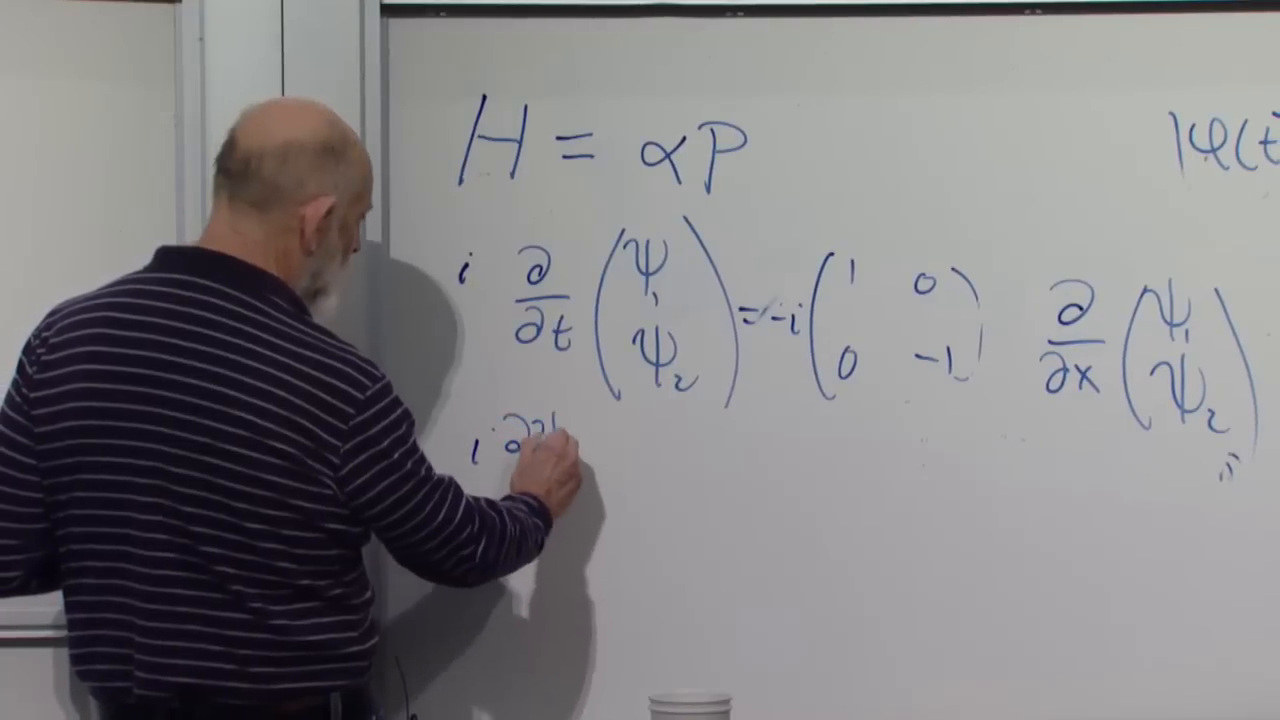
\includegraphics[width=0.94\linewidth]{lecture_09_frame_03.png}
\caption{黑板上的無質量二分量方程：\(H=\alpha P\)；對角矩陣為 \(\psi_1\) 和 \(\psi_2\) 指定相反的傳播方向。}
\lectureframe{01:26:00}
\end{figure}

單向傳播的問題解決了。負能量譜依然存在，而且我們又發現了第三個缺陷：兩個分量仍然沒有質量，並以光速傳播。接下來必須引入靜止能量，並將兩個方向耦合起來。

\section{加入質量並發現狄拉克代數}

加入一個最一般的簡單質量正比項，
\begin{equation}
H=\alpha p+\beta m,
\label{eq:l9-dirac-hamiltonian}
\end{equation}
其中 \(\beta\) 只作用於二分量指標。它可以是單位矩陣，也可以是其他矩陣；由相對論性色散關係來決定。

由於 \(H^2\) 必須等於 \(p^2+m^2\)，將式~\eqref{eq:l9-dirac-hamiltonian}平方：
\begin{align}
H^2
&=(\alpha p+\beta m)^2\\
&=\alpha^2p^2+\beta^2m^2
+(\alpha\beta+\beta\alpha)pm.
\label{eq:l9-square-dirac}
\end{align}
這些矩陣與 \(p\) 對易，因為它們作用於內部的二分量空間，而 \(p\) 作用於空間波函數。要符合式~\eqref{eq:l9-rel-dispersion}，必須滿足
\begin{equation}
\alpha^2=\mathbb{1},
\qquad
\beta^2=\mathbb{1},
\qquad
\{\alpha,\beta\}
=\alpha\beta+\beta\alpha=0.
\label{eq:l9-dirac-algebra}
\end{equation}
對 \(\alpha=\sigma_3\) 而言，第一個條件已經成立。任何不同的泡利矩陣都與它反對易，而且平方為單位矩陣。選擇
\begin{equation}
\beta=
\begin{pmatrix}
0&1\\
1&0
\end{pmatrix}
=\sigma_1.
\label{eq:l9-beta}
\end{equation}
選 \(\sigma_1\) 而不選 \(\sigma_2\) 是基底慣例；經過么正基底變換後，兩者實現的是相同的代數。

\begin{classroomqa}
\lecturetimestamp{01:33:00}
\audiencequestion{狄拉克只是看出泡利矩陣滿足這些代數條件嗎？}
\lecturerresponse{歷史上的推導是在三維中直接進行，並引入滿足所需關係的矩陣。寫出這些條件後，利用泡利代數便能立即得到一維解：選取兩個不同的泡利矩陣。}
\end{classroomqa}

\begin{classroomqa}
\lecturetimestamp{01:34:24}
\audiencequestion{這個 \(\beta\) 是相對論中的速度參數 \(v/c\) 嗎？}
\lecturerresponse{不是。它是作用於旋量分量的矩陣。字母重複使用只是狄拉克的記號，與運動學量 \(v/c\) 無關。}
\end{classroomqa}

在三個空間維度中，\(2\times2\) 矩陣不足以構成所需反對易矩陣的完整集合。這部分留待之後處理。在一維中，式~\eqref{eq:l9-alpha}和\eqref{eq:l9-beta}已經足夠。

\section{耦合的一維狄拉克方程}

代入 \(p=-i\partial_x\)，得到哈密頓形式的一維狄拉克方程：
\begin{equation}
i\partial_t\Psi
=\left(-i\alpha\partial_x+\beta m\right)\Psi.
\label{eq:l9-one-dimensional-dirac}
\end{equation}
由於 \(\alpha\) 是對角矩陣，導數項會讓兩個分量各自保持分離；由於 \(\beta\) 是非對角矩陣，質量項會使兩個分量互相轉換。逐分量寫成
\begin{align}
i\partial_t\psi_1
&=-i\partial_x\psi_1+m\psi_2,
\label{eq:l9-dirac-component-one}\\
i\partial_t\psi_2
&=+i\partial_x\psi_2+m\psi_1.
\label{eq:l9-dirac-component-two}
\end{align}

\begin{figure}[htbp]
\centering
\includegraphics[width=0.94\linewidth]{lecture_09_frame_08.png}
\caption{黑板上的耦合分量方程。導數項中相反的符號代表右行與左行；非對角的質量項則使 \(\psi_1\) 和 \(\psi_2\) 互相轉換。}
\lectureframe{01:37:44}
\end{figure}

只要 \(m\ne0\)，兩個分量就不再獨立演化。將一階方程平方後，每個分量都會得到克萊因--戈登算符：
\begin{equation}
\left(\partial_t^2-\partial_x^2+m^2\right)\psi_a=0,
\qquad a=1,2,
\end{equation}
平面波滿足 \(E^2=p^2+m^2\)，其群速度為
\begin{equation}
v_g=\frac{dE}{dp}=\frac{p}{E},
\end{equation}
只要質量不為零，群速度的大小就小於一。

質量與左右混合之間的關係並非偶然。無質量的右行粒子在任何正向洛倫茲變換下都仍是右行粒子；亞光速觀察者無法超越光，也就無法反轉它的方向。有質量的粒子可以被帶到靜止，再從沿同一方向運動且速度更快的參考系觀察；在該參考系中，粒子的速度看起來會反向。因此，有質量的相對論理論不可能讓右行與左行扇區永遠彼此隔離。非對角質量項恰好提供所需的耦合。

\begin{classroomqa}
\lecturetimestamp{01:40:01}
\audiencequestion{兩個分量互相轉換，這算是手徵振盪嗎？}
\lecturerresponse{在這個一維基底中，\(\alpha\)區分兩個無質量的手徵方向。質量項是非對角的，會使兩者混合，因此手徵性不再守恆。就此而言，質量項是手徵振盪的來源。}
\end{classroomqa}

\begin{classroomqa}
\lecturetimestamp{01:40:46}
\audiencequestion{為什麼費米子方程應該是玻色子方程的平方根？}
\lecturerresponse{不應該這樣理解。色散關係 \(E^2=p^2+m^2\) 適用於所有自由相對論粒子，不受統計性質影響。狄拉克算符恰好提供克萊因--戈登算符的矩陣分解，但這種代數關係並不能從玻色子推導出費米子。}
\end{classroomqa}

\begin{classroomqa}
\lecturetimestamp{01:41:31}
\audiencequestion{能否將方程化為簡單的純量分解，分別得到左行與右行因子？}
\lecturerresponse{只有在無質量極限下，兩個手徵方程才會解耦，成為彼此獨立的純量因子。當 \(m\ne0\) 時，有用的分解是矩陣值分解：反對易的 \(\alpha\) 與 \(\beta\) 矩陣正是消去多餘交叉項的關鍵。}
\end{classroomqa}

\begin{classroomqa}
\lecturetimestamp{01:42:04}
\audiencequestion{這兩個耦合方程已經構成狄拉克方程了嗎？}
\lecturerresponse{是的。兩式合起來就是一維空間中的狄拉克方程，也可以寫成式~\eqref{eq:l9-one-dimensional-dirac}的緊湊形式。乘上 \(\beta\) 可得到更對稱的協變記法，但這種寫法留待之後討論。}
\end{classroomqa}

還有兩項工作刻意留待後續處理。這個構造沒有消除負能量；它在兩個方向扇區中都提供了負能量解，因此這個問題反而更為明顯。而且理論仍然局限於一個空間維度。接下來要解釋負能量解，並將矩陣代數擴充到 \(3+1\) 維。
